% Options for packages loaded elsewhere
\PassOptionsToPackage{unicode}{hyperref}
\PassOptionsToPackage{hyphens}{url}
%
\documentclass[
]{article}
\usepackage{amsmath,amssymb}
\usepackage{lmodern}
\usepackage{ifxetex,ifluatex}
\ifnum 0\ifxetex 1\fi\ifluatex 1\fi=0 % if pdftex
  \usepackage[T1]{fontenc}
  \usepackage[utf8]{inputenc}
  \usepackage{textcomp} % provide euro and other symbols
\else % if luatex or xetex
  \usepackage{unicode-math}
  \defaultfontfeatures{Scale=MatchLowercase}
  \defaultfontfeatures[\rmfamily]{Ligatures=TeX,Scale=1}
\fi
% Use upquote if available, for straight quotes in verbatim environments
\IfFileExists{upquote.sty}{\usepackage{upquote}}{}
\IfFileExists{microtype.sty}{% use microtype if available
  \usepackage[]{microtype}
  \UseMicrotypeSet[protrusion]{basicmath} % disable protrusion for tt fonts
}{}
\makeatletter
\@ifundefined{KOMAClassName}{% if non-KOMA class
  \IfFileExists{parskip.sty}{%
    \usepackage{parskip}
  }{% else
    \setlength{\parindent}{0pt}
    \setlength{\parskip}{6pt plus 2pt minus 1pt}}
}{% if KOMA class
  \KOMAoptions{parskip=half}}
\makeatother
\usepackage{xcolor}
\IfFileExists{xurl.sty}{\usepackage{xurl}}{} % add URL line breaks if available
\IfFileExists{bookmark.sty}{\usepackage{bookmark}}{\usepackage{hyperref}}
\hypersetup{
  pdftitle={Planes, Trains, and Armored Mobiles: Introducing a Dataset of the Global Distribution of Military Capabilities (rDMC)},
  hidelinks,
  pdfcreator={LaTeX via pandoc}}
\urlstyle{same} % disable monospaced font for URLs
\usepackage[margin=1in]{geometry}
\usepackage{longtable,booktabs,array}
\usepackage{calc} % for calculating minipage widths
% Correct order of tables after \paragraph or \subparagraph
\usepackage{etoolbox}
\makeatletter
\patchcmd\longtable{\par}{\if@noskipsec\mbox{}\fi\par}{}{}
\makeatother
% Allow footnotes in longtable head/foot
\IfFileExists{footnotehyper.sty}{\usepackage{footnotehyper}}{\usepackage{footnote}}
\makesavenoteenv{longtable}
\usepackage{graphicx}
\makeatletter
\def\maxwidth{\ifdim\Gin@nat@width>\linewidth\linewidth\else\Gin@nat@width\fi}
\def\maxheight{\ifdim\Gin@nat@height>\textheight\textheight\else\Gin@nat@height\fi}
\makeatother
% Scale images if necessary, so that they will not overflow the page
% margins by default, and it is still possible to overwrite the defaults
% using explicit options in \includegraphics[width, height, ...]{}
\setkeys{Gin}{width=\maxwidth,height=\maxheight,keepaspectratio}
% Set default figure placement to htbp
\makeatletter
\def\fps@figure{htbp}
\makeatother
\setlength{\emergencystretch}{3em} % prevent overfull lines
\providecommand{\tightlist}{%
  \setlength{\itemsep}{0pt}\setlength{\parskip}{0pt}}
\setcounter{secnumdepth}{5}
\usepackage{tikz}
\usepackage{pgfplots}
\pgfplotsset{compat=newest}
\usetikzlibrary{plotmarks}
\usetikzlibrary{arrows.meta}
\usepgfplotslibrary{patchplots}
\usepackage{grffile}
\usepackage{caption}
\usepackage[utf8]{inputenc}
\usepackage[doublespacing]{setspace}
\usepackage{float}
\usepackage{multirow}
\ifluatex
  \usepackage{selnolig}  % disable illegal ligatures
\fi
\newlength{\cslhangindent}
\setlength{\cslhangindent}{1.5em}
\newlength{\csllabelwidth}
\setlength{\csllabelwidth}{3em}
\newenvironment{CSLReferences}[2] % #1 hanging-ident, #2 entry spacing
 {% don't indent paragraphs
  \setlength{\parindent}{0pt}
  % turn on hanging indent if param 1 is 1
  \ifodd #1 \everypar{\setlength{\hangindent}{\cslhangindent}}\ignorespaces\fi
  % set entry spacing
  \ifnum #2 > 0
  \setlength{\parskip}{#2\baselineskip}
  \fi
 }%
 {}
\usepackage{calc}
\newcommand{\CSLBlock}[1]{#1\hfill\break}
\newcommand{\CSLLeftMargin}[1]{\parbox[t]{\csllabelwidth}{#1}}
\newcommand{\CSLRightInline}[1]{\parbox[t]{\linewidth - \csllabelwidth}{#1}\break}
\newcommand{\CSLIndent}[1]{\hspace{\cslhangindent}#1}

\title{\singlespacing Planes, Trains, and Armored Mobiles: Introducing a Dataset of the Global Distribution of Military Capabilities (rDMC)}
\author{Belfer Center for Science and International Affairs\\
Harvard Kennedy School\\
\hspace*{0.333em}J Andr\(\'{e}\)s Gannon\footnote{Email: \texttt{jagannon@hks.harvard.edu}. Web: \texttt{jandresgannon.com}. \newline See \texttt{https://www.militarycapabilities.com/} for a website of the complete project. Data and code for the empirical analysis can be found at \texttt{https://github.com/CenterForPeaceAndSecurityStudies/rDMC}. This projected was funded and produced by the UC San Diego Center for Peace and Security Studies.}}
\date{May 05, 2022}

\begin{document}
\maketitle
\begin{abstract}
\singlespacing \noindent This article introduces the Distribution of Military Capabilities (rDMC) dataset. It begins by explaining the value of collecting data on disaggregated national military capabilities, its scope, and the data collection process. I then identify some initial trends about changes in the distribution of military capabilities across states from 1970 -- 2014. I conclude by identifying future research use of the data as both a dependent and independent variable.
\end{abstract}

\newpage

\hypertarget{introduction}{%
\section{Introduction}\label{introduction}}

The military capabilities states possess are an important instrument of military power, and consequently national power (Morgenthau 1948). Yet existing work on both the causes and consequences of military power are limited in empirical identification to coarse measures like military spending or military personnel. Not all soldiers are created equal, and much has been said about the problems of measuring military power using military spending figures (Perlo-Freeman 2017) or aggregate measures like the composite index of national capabilities (CINC) (Carroll and Kenkel 2019). While military technology is one of only many components of military power (and military equipment only one dimension of military technology), its effects are significant, if hotly debated. Without denying the importance of non-technological factors like military culture, institutions and doctrine (Lieber 2005; R. Brooks and Stanley 2007), inconsistent findings about the role of technology in conflict stem not from the fact that technology does not matter, but rather it has been improperly identified and coarsely measured (van Creveld 2010; S. G. Brooks and Wohlforth 2016).

This paper seeks to contribute to ongoing research about the causes and consequences of military power by producing the first comprehensive dataset of the distribution of military capabilities across all states from 1970 -- 2014. Disaggregating military power into its component parts is an important, yet underdeveloped, enterprise. While aggregate military spending may help differentiate large and globally capably militaries from smaller ones, it risks conflating differences in the \textit{composition} of nominally equivalently sized militaries. The composition of a state's navy may influence its threats, power projection, and warfighting capabilities in some conflicts, but not others (Caverley and Dombrowski 2020; Gartzke and Lindsay 2020), and the relationship between the military technologies a country could acquire, actually possesses, and subsequently uses in a contest could shed light on contrasting findings about the impact of military capabilities on international affairs (Douglass and Gannon 2019).

This paper proceeds as follows. Section 2 identifies the role that military technology plays as both an important cause and consequence in the study of international politics. Section 3 outlines the scope of the newly produced Distribution of Military Capabilities (rDMC) dataset. Section 4 briefly describes the data collection process. Section 5 identifies some initial trends in variation in the distribution of military capabilities across time and space and Section 6 concludes.

\hypertarget{significance}{%
\section{Significance}\label{significance}}

Most of the research on international conflict has focused on the beginning and end of war -- its causes and consequences. However, the conduct of conflict, whether actual or latent, has much to tell us about war's causes and consequences (Boot 2006; Biddle 2007). Regarding its causes, if, as Clausewitz noted, war is the continuation of politics with other means, then the tools used for war \textit{are} the other means. Military means \textit{might} matter, but evaluating whether they do (and if so, the degree and circumstance) is an impossible endeavor without empirical data on the distribution of those means across time and space. If it turns out that military means do matter, then Clausewitz's point is that understanding these means fundamentally shapes our understanding of war as a political process. What a country is able to accomplish with military force in a specific situation is a function of military technology, organization, and doctrine and the manner in which these things relate with the political and geographic circumstances at hand (Betts 1997). Regarding war's consequences, the military capabilities available to actors play a role in determining whether bloodshed is preferable to resolving the dispute through a negotiated settlement (Slantchev 2003b).

The innovation, acquisition, and organization of military technology is an important determinant of national military force since it comprises the tools available for the resolution of international disputes. The combination of capabilities that comprise a military's toolkit determine the operations it undertakes, the types of threats it can credibly make, and the consequences of resorting to force (Buzan 1987). In other cases, military technology has had contrasting consequences in the same conflict despite prior expectations of consistency. During the 1879 Anglo-Zulu War, the United Kingdom expected their firearms -- and the lack of any Zulu contact with firearms -- to provide a significant tactical advantage (Guy 1971). However, the United Kingdom suffered a serious loss at Isandlwana despite being armed with the Martini-Henry rifle (Beckett 2013). After this resounding defeat, the British shifted their technological strategy by deploying the recently invented Gatling gun which allowed the much smaller British army to overwhelm the Zulu tribes in a matter of minutes Willbanks (2004, 33). Two cases of technological superiority were associated with contrasting outcomes, pointing to the importance of identifying different types of technology in warfare rather than just the presence of innovation.

The wide body of literature studying war has recognized the degree to which these concerns are shaped by \textit{how} states fight. If scholars understand the process by which states make choices about what military capabilities they possess, they can better understand how different aspects of those capabilities impact outcomes of interest (Caforio 2006). The tools that comprise national military force influence war's participants (Fordham 2004; Beckley 2017), victors (Rosen 1991; Lyall and Wilson 2009; Cappella Zielinski and Grauer 2020), costs (Caverley 2014; Talmadge 2019), location (Schilde 2017; Crisher 2017), and duration (Martinez Machain 2015; Cappella Zielinski 2016b; Caverley and Sechser 2017) as well as power projection (Corbett 1911; Beasley 2015), what issues are resolved with force (Allison and Morris 1975; Becker 2017), what threats are credible (Buzan and Herring 1998; Slantchev 2003a; Post 2019; Montgomery 2020), reputation (Erickson 2018), and the balance of power (Glaser 1992; Horowitz 2010; Gartzke, Kaplow, and Mehta 2014).

The portfolio of military capabilities also informs broader questions outside the traditional scope of international security like when coups succeed (Talmadge 2016; Caverley and Sechser 2017) and civil-military relations (Forster 2005; R. Brooks 2008; Kadercan 2014). In the early 1972, the head of the Bangladeshi government successfully held off a coup by creating a special security force (the Jatio Rakkhi Bahini) of loyal forces. Two years later, however, Bangladesh purchased 30 T-54 tanks from Pakistan which allowed the army to overtake the special security forces in a storm of the president's residence, resulting in his death and an overthrow of the secular government (Maniruzzaman 1992, 745--47).

The study of domestic politics has also recognized the importance of military capabilities. Tension between political budget constraints and military security desires gets to the heart of the role that military capabilities play in furthering our understanding of national politics (Fordham 2004; Cappella Zielinski 2016a; Gholz and Sapolsky 2020). Other domestic issues like inter-branch relations (Jones and Marsh 2011), public opinion (E. N. Saunders 2015), and interest group lobbying (Holland 1993; Dombrowski and Gholz 2006; Gholz 2011) all point to the importance of a better understanding of the drivers of a state's military portfolio.

Despite the shortcomings of aggregate measures for explaining concepts of interest, most current research still focuses on variation in the \textit{size} of state militaries (Aufrant 1999; Fordham 2002; Sample, Valeriano, and Kang 2013; Cappella Zielinski, Fordham, and Schilde 2017; Odehnal and Neubauer 2020). Recent work that disaggregates military technology has investigated the relationship between important conflict outcomes and capabilities like naval platforms (Crisher and Souva 2014), mechanized armies (Lyall and Wilson 2009; Sechser and Saunders 2010), and air power (Martinez Machain 2015; Allen and Martinez Machain 2017, 2018; R. Saunders and Souva 2020). Despite these data being limited in scope, this existing research highlighted the value of disaggregating military power for understanding the international balance of power.

National militaries are primarily quantified and compared by military spending levels or, in rarer cases, military personnel counts. Yet data on military spending poses known problems as a metric for cross-national and temporal comparison (Perlo-Freeman 2017). Since there are no common definitions about what constitutes military spending, some states measure things like pension and R\&D while others do not (Amara and Paskevics 2010). Exchange rates are often used to standardize all spending to the same currency, but with ill-information applications of domestic purchasing power (Fontanel 1996). Factors like inflation and varying budget cycles are also difficult to account for and dramatically impact inferences drawn from different data sources (Lebovic 1999). Sources like the IMF, the UN Office for Disarmament Affairs, the US Bureau of Arms Control, Verification, and Compliance, the International Institute for Strategic Studies (IISS), and the Stockholm International Peace Research Institute (SIPRI) all produce annual military spending estimates but they use different estimating procedures, primary sources, and preparation methods (Brzoska 1981), meaning theories supported using one data source will often not be supported using comparable data from another source (Boniface 1995).

Military spending data also has a temporal bias, with earlier time periods experiencing higher uncertainty. This has been extensively documented in the case of West Germany military spending during the Cold War, where later research found that West Germany's internal figures differed from what they were reporting to NATO (Brzoska 1981; Cowen and Karp 1986). Even commonly used sources like SIPRI caution researchers on using their military spending data for cross-national comparisons, arguing that it is instead only appropriate to compare any one country over time (Omitoogun and Skons 2006). Furthermore, military spending measures don't account for what states spend that money on and how variations in factors like geography complicate our ability to compare the production of security across states. While these problems likely exist with military equipment data as well, scholars have not even been able to identify the degree or direction of this bias because the data does not yet exist.

Measurement issues aside, although scholars and practitioners know that defense spending varies across space and time, a second dimension of important and understudies variation is that militaries also vary in their \textit{composition}.\footnote{Of course, these two are not synonymous. Military capabilities are only one component of military spending and the cost of labor is a large component of military spending (Fordham 2002; Whitten and Williams 2011).} Scholars have noted ``there is a lack of knowledge about variation between states in their behavior on armaments policy decisions" (Mawdsley 2018) because of problems empirically identifying the military capabilities states possess (Fordham 2004). But in order to identify the drivers of armament decisions, scholars must know what armament decisions have been made (Kurth 1973). Understanding differences in the composition of military capabilities is vital to understanding military power because these components are not homogeneous. These capabilities differ in what they can accomplish (Lindsay and Gartzke 2020) and the fact there are differences in how even similarly-sized states arm themselves is prima facie evidence of the non-fungibility of material military power. Military spending itself does not create military power; rather, that money must be translated into capabilities that allow for the exercise of power through a variety of distinct means.

Although scholars of international conflict have paid comparatively little attention to identifying the distribution of military capabilities, the same is hardly true for practitioners. During the Cold War, British diplomat James Cable (1970, 127) described the US as ``the only navy with the sheer number of ships, with enough aircraft carriers, ocean-going surface warships, amphibious craft and supply vessels, to undertake every class of operation, in any part of the oceans and for as much of the future as can yet be foreseen.'' This is the political dimension of force structure decisions -- what a states produces and omits in its defense portfolio reflects its political priorities in ways that economic considerations alone cannot explain (Hone 1993; Caverley 2007). As then-Senator Joseph Biden (2008) remarked regarding domestic economic policy during his vice presidential campaign, ``{[}d{]}on't tell me what you value. Show me your budget, and I'll tell you what you value.'' This also holds true in the military context, where disconnects concerning a state's budget and alleged priorities are missed by looking at top-line spending figures. Despite decades of concern about a Chinese invasion of Taiwan, it was not until 2017 that China began investing in the amphibious assault capabilities that are necessary for that threat to actually be carried out (Office of the Secretary of Defense 2018, 95--99).

\hypertarget{the-rdmc-dataset-scope-and-data-generating-process}{%
\section{The rDMC Dataset: Scope and Data Generating Process}\label{the-rdmc-dataset-scope-and-data-generating-process}}

This paper introduces the first comprehensive dataset of disaggregated military capabilities. Data on military technology portfolios is produced by the International Institute for Strategic Studies (IISS) in the annual Military Balance reports. Different portions of these reports have been used frequently in academic publications. Most of this work has used IISS data on military spending (Goldstein 1998; Wohlforth 1999; Hallerberg and Marier 2004; Greenhill and Major 2007) or personnel (Lieber and Alexander 2005; Sundstrom 2005; Walter 2006; Stanton 2013; Gaibulloev et al. 2015). The little work that has looked at IISS data on the distribution of military capabilities has focused on a narrow list of platforms like mechanized vehicles (Lyall and Wilson 2009; Sechser and Saunders 2010), strategic lift aircraft (Kupchan 1988), and fighter jets (R. Saunders and Souva 2020) or a short list of countries like great powers (S. G. Brooks and Wohlforth 2016) or China and its rivals (Beckley 2017). The primary reason for this relatively limited use of fine-grained high-quality data is difficulty in converting the data to an easily-usable format and standardizing it across countries and years.

The data represent military capabilities for 184 countries over almost half a century (1970 -- 2014). Although the Military Balance was first published in 1961, prior to 1970 the report focused on NATO and Warsaw Pact states only, with more information provided about the former than the latter (Nelson 1985; Böhmelt and Pilster 2015). Using 1970 as the cut off, Figure \ref{fig:missingness} shows what percent of years are coded for each country.\footnote{I use percent of years since not all countries exist across the entire duration of the data. 100\% of Slovenia is covered, for example, because data exists for all 22 years since since it established independence in 1991.} 54\% of countries have no missing data across the entire time span, with the median country having data available for 95\% of its years and the mean country having 88\% coverage.

\begin{figure}[H]

{\centering 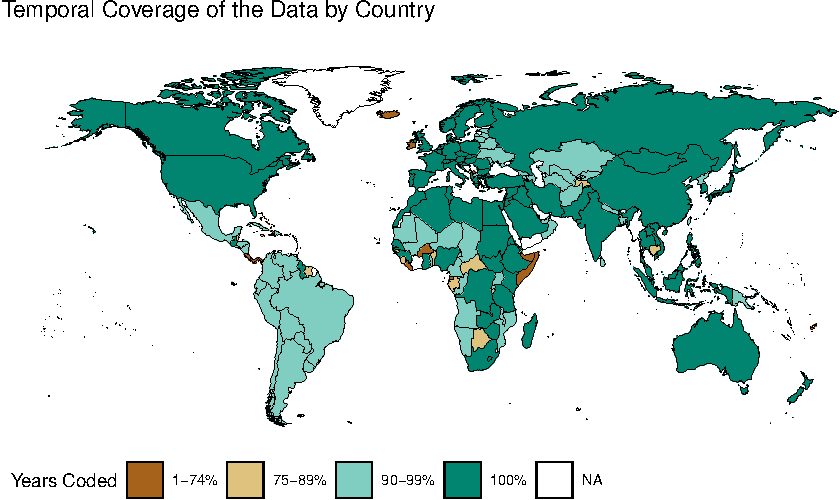
\includegraphics{2021-10-05_rDMC_files/figure-latex/missingness-1} 

}

\caption{Coverage of available data on state military capabilities (1970 -- 2014)}\label{fig:missingness}
\end{figure}

The military capabilities are organized hierarchically, with higher levels of organization representing broad categories like helicopters or principal surface combatants and lower levels of organization representing distinct roles within those categories like attack helicopters versus transport helicopters or aircraft carriers versus destroyers. The rDMC codebook accompanying this paper and dataset describes the temporal and spatial scope of the data as well as the military capabilities that are included.

As with much data in international affairs, concerns about data quality and accuracy remain salient. The extensive use of the IISS Military Balance reports by other scholars gives some confidence in its accuracy and also allows for the data codings here to be double-checked with data codings by other scholars to correct data entry and coding errors. An extensive, but not exhaustive list of those publications is provided in the appendix. A list of the most comprehensive uses of IISS military capabilities data is provided in Table \ref{table:iiss_litreview}.

\begin{singlespace}
    \begin{table}[h]
      \centering
      \caption[Prior use of IISS data]{Sample of the 10 most comprehensive uses of IISS military equipment data in major political science publications (listed chronologically). A full list of all 20 documented publications, including the list of countries and years used, is available from the author.}
      \begin{tabular}{|p{5.5cm}|c|c|p{6cm}|}
            \hline 
            \textbf{Publication} & \textbf{Years} & \textbf{Countries} & \textbf{Technologies} \\ 
            \hline 
            Haesebrouck (2018) & 1 & 43 & Combat aircraft \\ 
            \hline 
            Beckley (2017) & 20 & 9 & Submarines, surface ships, 4th generation fighter aircraft \\ 
            \hline 
            Kang (2017) & 1 & 32 & Naval vessels \\ 
            \hline 
            Brooks (2016) & 1 & 6 & Submarines, aircraft carrier, combat ships, UAVs, tactical aircraft, satellites, aircraft, helicopters \\ 
            \hline 
            Sandler (2014) & 1 & 31 & Combat aircraft \\ 
            \hline 
            Sechser (2010) & 11 & 150 & Armored vehicles \\
            \hline
            Lyall (2009) & 1 & 167 & Mechanized vehicles \\ 
            \hline
            Auerswald (2004) & 1 & 5 & Aircraft \\ 
            \hline 
            Posen (2003) & 2 & 1 & Ships and aircraft \\ 
            \hline 
            Kupchan (1998) & 6 & 5 & Strategic lift aircraft \\ 
            \hline 
        \end{tabular} 
        \label{table:iiss_litreview}
    \end{table}
    \end{singlespace}

Policymakers similarly rely on the IISS Military Balance reports, with former US Army General Petraeus describing it as ``the go-to source of unclassified, independent information on defense capabilities around the world,'' former US Secretary of Defense Robert Gates noting that it ``provides essential facts and analysis for decision-makers and for better informed public debate,'' and former US Secretary of Defense Leon Panetta remarking that it is ``widely recognised as the best unclassified source of defense information on personnel, equipment and budgets for every country.'' Even if the data does not perfectly represent state military capacities, it influences how policymakers behave since they use the data for their analysis. The former Supreme Allied Commander of NATO, Admiral James Stavridis, said ``throughout my career, I have relied extensively on The Military Balance produced so expertly by the IISS. It is the ``go to'' source for serious analysts and warriors facing real world challenges."\footnote{Quotes come from \href{https://www.iiss.org/publications/the-military-balance}{IISS Testimonials}}

The accuracy of the data can also be double checked in certain instances using reliable primary source data from government reports. New Zealand, for example, publishes annual reports on the military's performance targets that describe the resources at the military's disposal (Alexander, King, and Robert 2002). Although such data is not available for all countries nor for all years, checking the data in such a manner where possible should provide face validity about the accuracy of the IISS measures.

\hypertarget{data-collection-and-formats}{%
\section{Data Collection and Formats}\label{data-collection-and-formats}}

The data collection process first involved creating a consistent typology of military equipment types, equipment names, and unit names. I create two versions of the data. The first, \textit{rDMC raw}, organizes military equipment true to the original IISS categorizations. The second and third, \textit{rDMC long} and \textit{rDMC wide} produce a new more aggregated classification of military capabilities. Table \ref{table:categories} shows the unique values that exist at each nested level in the categorization scheme provided by IISS, how that can be aggregated using IISS categories, and then how that is further aggregated in the final classification. A detailed description of the different data versions follows.

\begin{singlespace}   
    \begin{table}[h]
        \centering              
        \caption[Categories of military capabilities]{Description of unit of analysis and variables in the different versions of the rDMC dataset.}
    \begin{tabular}{|c|c|c|c|}
            \hline
            \textbf{Data Version} & \textbf{Unit of Analysis} & \textbf{N} & \textbf{Variables} \\
            \hline
            Raw & Country-year-unit & $356,096$ & Service, disaggregated categories, count \\
            \hline
            Long & Country-year-tek & $475,302$ & Aggregate category, count \\
            \hline
            Wide & Country-year & $6,534$ & Technologies \\
            \hline
        \end{tabular}
        \label{table:categories}
    \end{table}
    \end{singlespace}

\hypertarget{rdmc-raw}{%
\subsection{rDMC raw}\label{rdmc-raw}}

IISS categorizes military capabilities according to the following levels, in order of increased specificity: equipment types, equipment subtypes, equipment names, equipment subnames, and unit names.\footnote{While these 5 classifications levels are produced by IISS, their labels are the author's.} Equipment type involves the most aggregate categorizations like aircraft or armored fighting vehicles. Subtype and subname are auxiliary classifications that exist for some, but not all technologies, like designations of light, medium, and heavy variations of transport aircraft or distinguishing difference classes of aircraft carriers. Equipment names are the next primary IISS categorization and produce information about classifications like transport or fighter aircraft or main battle tanks as a variety of armored fighting vehicles. Then at the unit level one can identify, for example, the number of M1A1 Abrahms main battle tanks each country possessed.

The main utility of the \textit{rDMC raw} categorization is in providing an objective and unaltered version of the original IISS data, true to their data generating process. No coding decisions, new equipment categorizations, or ontologies inform this version of the data. Furthermore, this version of the data is unique in providing unit-level information. This level of disaggregation has potential use for studies examining questions like combat effectiveness, arms sales, or interest group lobbying.\footnote{Matching various unit name string variables is a challenging endeavor. For more information about using the unit-level information in \textit{rDMC raw}, see the appendix.}

For example, scholars have identified the challenges of observable proxies for ex-ante military effectiveness (R. Brooks and Stanley 2007; Millett and Murray 2010a, 2010b, 2010c). Biddle (2005, 135) uses the age of military technology as a proxy for its effectiveness. During Operation Desert Storm, the average date of introduction for US weapons was 1974 while Iraq's was 1962. But until now, broader measures of the age of different components of a state's military portfolio have remained unexamined. Scholars interested in dependent variables like military effectiveness could use this information to differentiate the predicted battlefield performance of a state with 100 M1A2 SEPv2 Abrams main battle tanks (in service since 2013) with a state with 100 T-55 main battle tanks (in service since 1949). As an example, Figure \ref{fig:mbt-invention} shows a broader comparison of the age of introduction for each main battle tank in the data as well as its last recorded year in service. The year of introduction is identified as the first year in which at least one state possessed that type of tank.\footnote{Since the data starts in 1970, tanks first deployed in 1970 actually likely represent models developed before then. A more thorough analysis would track down the actual deployment date for each tank model, rather than relying on their deployment date as done here.} Since data also exists about the origins and national producers of various military units, research on arms sales would benefit from being to more thoroughly identify patterns in reliance (Caverley et al. 2013; Erickson 2018).

\begin{figure}[H]

{\centering 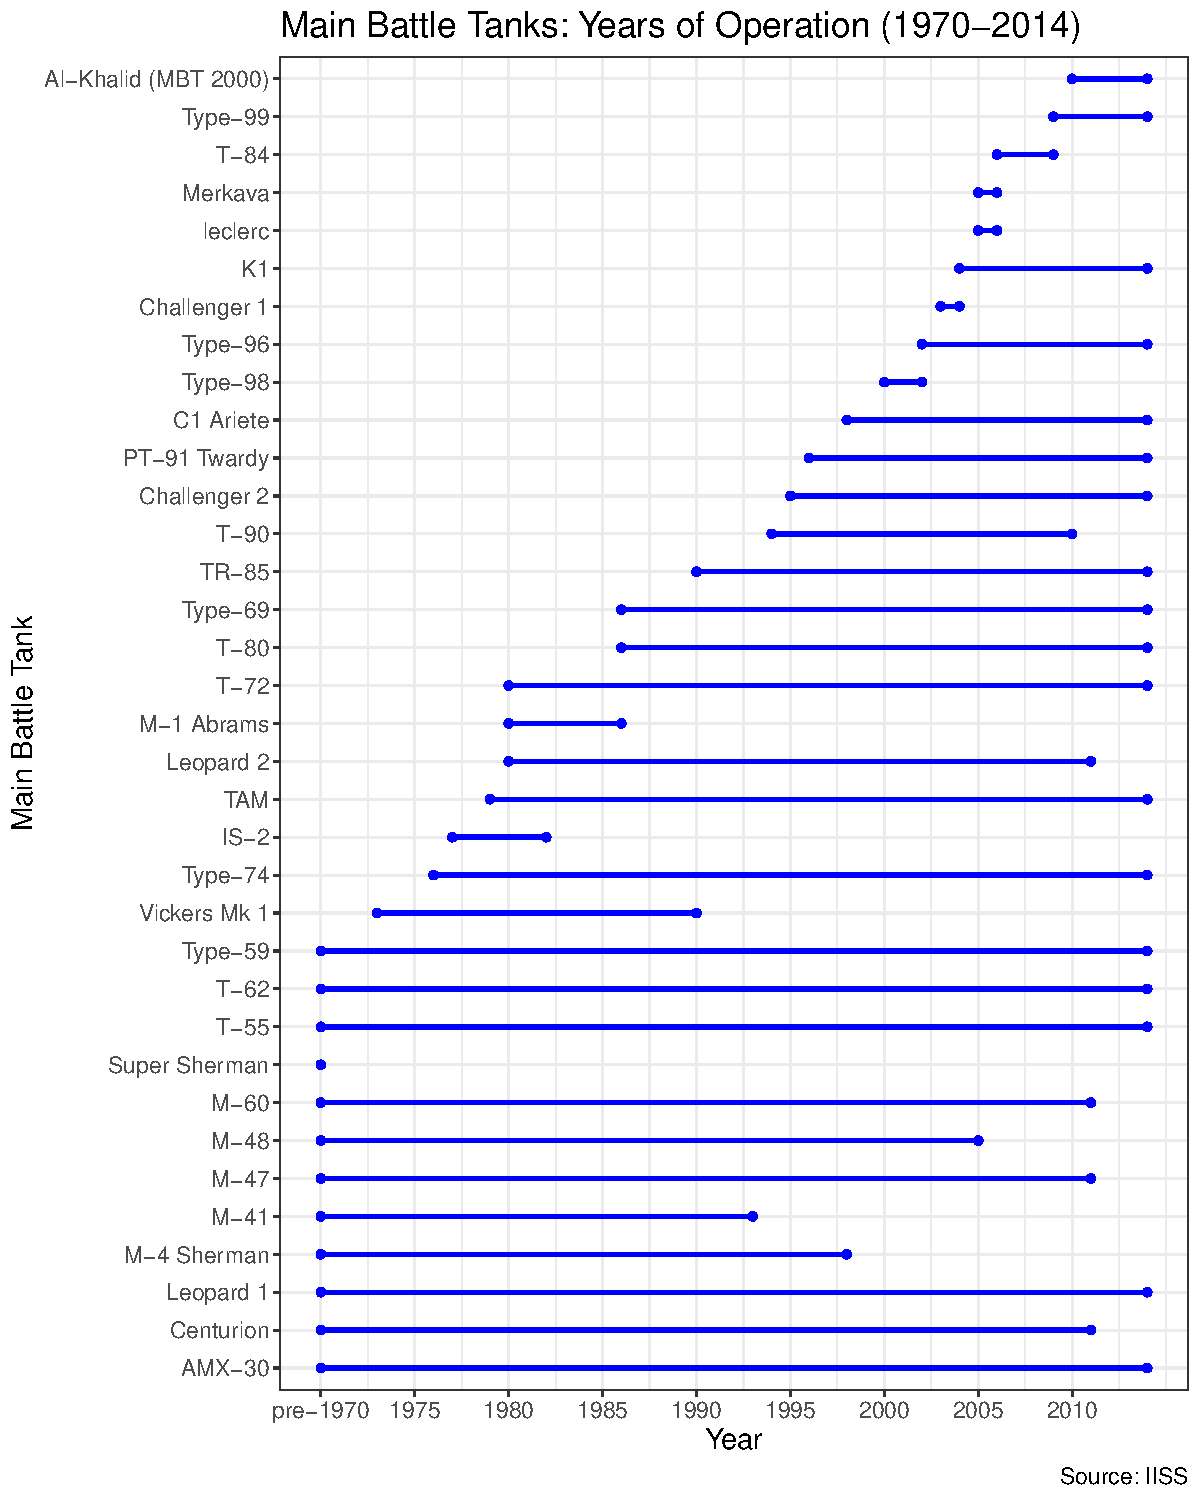
\includegraphics{2021-10-05_rDMC_files/figure-latex/mbt-invention-1} 

}

\caption{The first year in which each type of main battle tank was deployed by any state. The figure is organized chronologically, with the newest main battle tanks at the top.}\label{fig:mbt-invention}
\end{figure}

\hypertarget{rdmc-long-and-rdmc-wide}{%
\subsection{rDMC long and rDMC wide}\label{rdmc-long-and-rdmc-wide}}

From this, the technology categories are aggregated to a new typology representing variety in military technologies of interest to scholars who have less of a need for granular information differentiating M1A1 Abrahms tanks from M1A2 Abrahms tanks and are instead interest in the number of armored combat vehicles a state possesses. I first aggregated the technologies to unique triples composed of equipment type, subtype, and name using the IISS categorizations. This typology is consistent across country and year, thus simplifying the process of time series-cross sectional analysis. Where inconsistencies arise, coding decisions were made with reference to external sources and transparently coded in the data available online. This ensure that, for example, the C-130H Hercules is always listed with an equipment type coding of `aircraft' and an equipment name coding of `transport (TPT)'.\footnote{There are cases where an equipment's category changes in ways the data maintains. For example, many aircraft and helicopters are phased out by being shifted to non-combat roles like training before they are fully retired. A country may thus experience a decrease in combat aircraft and an increase in training aircraft from one year to the next without the actual aircraft they possess changing.} This results in a count for ``aircraft -- transport'' for every country with a value that is the sum of all units that country possessed that had the equipment type, subtype, name, subname, and unit name corresponding to that higher level aggregation.

\textit{rDMC long} and \textit{rDMC wide} are identical in terms of content and differ only in the unit of analysis. In \textit{rDMC long}, the unit of analysis is the country-year-technology, so the only variable for each row is the numeric count corresponding to the unique identifier. In \textit{rDMC wide}, the unit of analysis is the country-year with each unique technology value becoming its own column. Although both versions are substantively identical, both are provided as reshaped versions of each other to simplify the process of subsetting and merging with other datasets. Given their interchangeability, in the section that follows, either version can be used to produce substantively identical figures and summary statistics.

The 115 categories that comprise the technologies are shown in Figure \ref{fig:dendrogram}. Empirically, this aggregation is helpful because the technology categories are definitionally uniform across the data sample. Theoretically, these categories were chosen because they represent weapons categories commonly recognized and used by states in arms reduction agreements like the Treaty on Conventional Armed Forces in Europe (CFE). As a result, national records are most consistent and accurate at this level of analysis since those records were used during international negotiations.

Computationally, aggregating the technology categories also reduces the sparseness of a data set that is already zero-inflated. While most country-years possess armored fighting vehicles, not all possess every kind of armored fighting vehicle (main battle tanks, armored personnel carriers, armored infantry fighting vehicles, and reconnaissance vehicles) let alone each of the 1775 distinct units categorized as ``armored fighting vehicles.'' That is not to say that every type or model is the same; if it was then 6,000+ United States armored personnel carriers would not be split across 5 different models. But those distinctions present computational challenges given that even the militarily-capable United States possesses only a small fraction of all the different kinds of armored personnel carriers that exist. As a result, country-specific units would inflate inferences about between-country variation in military portfolios. Scholars interested in making those sorts of distinctions are advised to use the \textit{rDMC raw} version of the data.

\begin{figure}[H]

{\centering 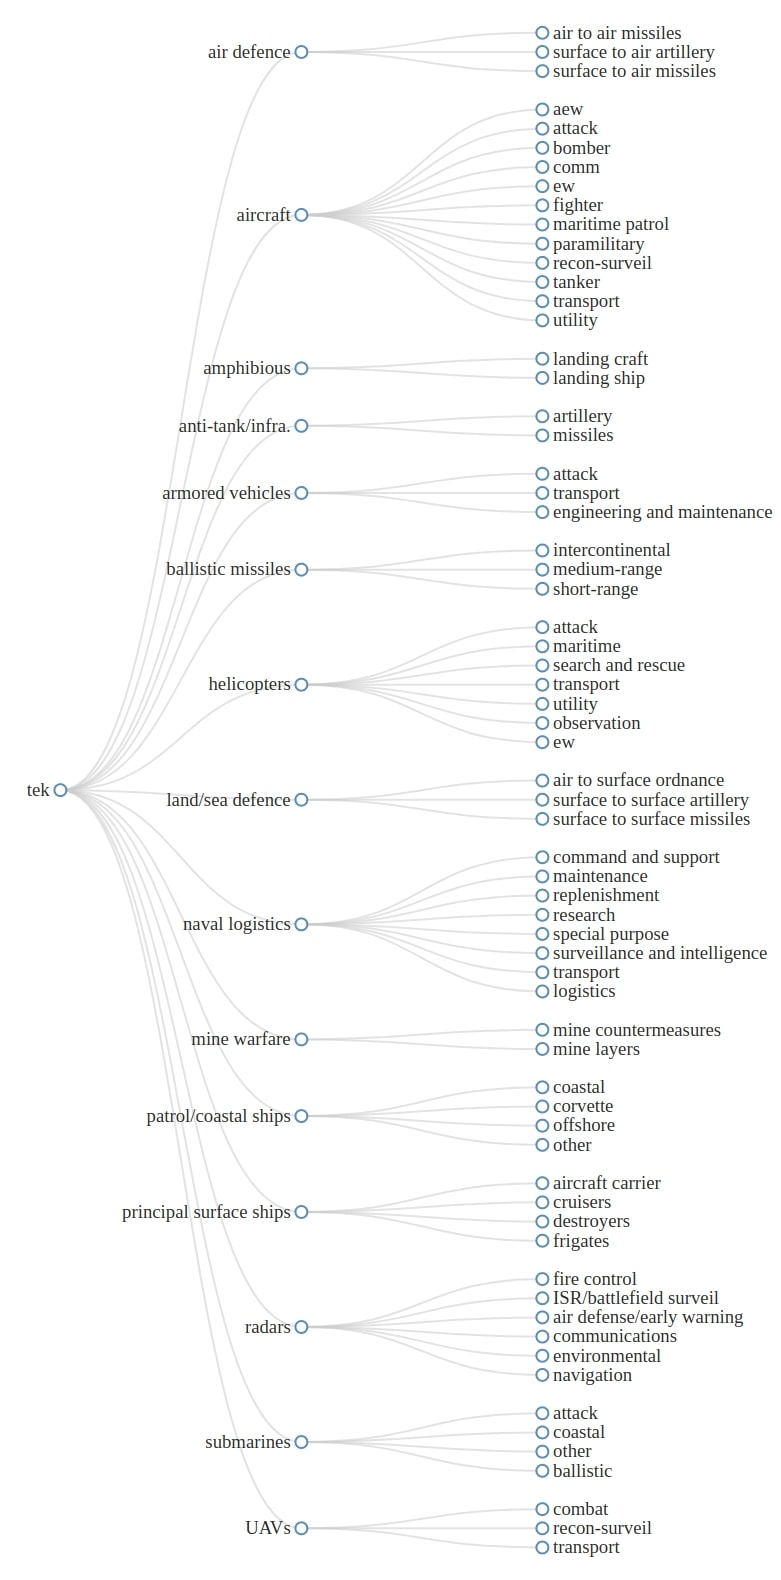
\includegraphics[width=1\linewidth,]{/home/andresgannon/Dropbox (rex)/Grad School/andres_github_private/rDMC/paper/dendrogram_subjective_full} 

}

\caption{Description of the aggregated technologies used to compute the distribution of military capabilities.}\label{fig:dendrogram}
\end{figure}

There are, of course, many ways to categorize technologies. Some categories could be grouped together depending on the research interest. ``Aircraft -- transport'' and ``helicopters -- transport'' could be considered somewhat interchangeable to those interested in a state's ability to move personnel and material via the air. Alternatively, ``helicopters -- transport'' could be grouped with ``helicopters -- search and rescue'' if studying a topic like arms sales or military base location given similarity in their physical make-up. Some categories could also be further \emph{dis}aggregated. The category ``aircraft -- maritime patrol,'' for example, include anti-submarine warfare, anti-surface warfare, and maritime reconnaissance which all ``patrol'' different areas of the sea. Aside from these deductive ways of aggregating or disaggregating the military technologies, inductive methods could identify different sets of similar technologies based on things like rarity, pairwise occurrence, or component parts (Douglass and Gannon 2019). Rather than try to create and justify a single definitive ontology of military technologies, the data are constructed so that all aggregations are transparent and, more importantly, modular. By simply selecting new aggregation categories, scholars can produce their own counts with different categories. Scholars who wish to differentiate between those categories can transparently see how those were aggregated, change those aggregations (including creating new technology categories or deleting existing ones), and produce a new dataset consistent with the classifications that suite their research questions.

\hypertarget{application}{%
\section{Application}\label{application}}

\hypertarget{conclusion}{%
\section{Conclusion}\label{conclusion}}

Heterogeneity in how states arm themselves exists and is significant both in terms of substance and consequence. Identifying the dimensions of this heterogeneity is a necessary precondition for explaining both its causes and consequences in international affairs. To date, explanations of the causes or effects of variation in the composition of a state's military assets has been empirically limited because that data has not existed in a way conducive to systemic analysis. This is not just true for quantitative scholars interested in large cross-national regressions; scholars studying individual countries, regions, or specific time periods have been limited in their ability to provide even descriptive accounts about the balance of military power using any observations more detailed than national military spending, military personnel counts, or outcomes of interests like actualized conflicts. The hope is that the broader scholarly community can use the data created here to answers other questions of interest. While much ink has been spilled debating \textit{whether} military technology matters (Tuchman 1962; Rosen 1991; Betts 1997), the discussion should productively shift to \textit{what} military technologies matter and \textit{how}. In transparently presenting the process by which this data was created, that should be easier.

\newpage

\hypertarget{references}{%
\section*{References}\label{references}}
\addcontentsline{toc}{section}{References}

\hypertarget{refs}{}
\begin{CSLReferences}{1}{0}
\leavevmode\hypertarget{ref-alexander_countrysurveyxvii_2002}{}%
Alexander, J., Alan B. King, and W. Robert. 2002. {``Country Survey {XVII}: {New} Zealand's Defence Policy.''} \emph{Defence and Peace Economics} 13 (4): 287--309. \url{https://doi.org/10.1080/10242690212355}.

\leavevmode\hypertarget{ref-allen_understandingimpactair_2017}{}%
Allen, Susan Hannah, and Carla Martinez Machain. 2017. {``Understanding the Impact of Air Power.''} \emph{Conflict Management and Peace Science} 36 (5): 545--58. \url{https://doi.org/10.1177/0738894216682485}.

\leavevmode\hypertarget{ref-allen_choosingairstrikes_2018}{}%
---------. 2018. {``Choosing {Air Strikes}.''} \emph{Journal of Global Security Studies} 3 (2): 150--62. \url{https://doi.org/10.1093/jogss/ogy005}.

\leavevmode\hypertarget{ref-allison_armamentsarmscontrol_1975}{}%
Allison, Graham T., and Frederic A. Morris. 1975. {``Armaments and {Arms Control}: {Exploring} the {Determinants} of {Military Weapons}.''} \emph{Daedalus} 104 (3): 99--129.

\leavevmode\hypertarget{ref-amara_unfulfilledpromisesimpact_2010}{}%
Amara, Jomana, and Martins Paskevics. 2010. {``Unfulfilled {Promises}: {The Impact} of {Accession} on {Military Expenditure Trends} for {New NATO Members}.''} \emph{Comparative Strategy} 29 (5): 432--49. \url{https://doi.org/10.1080/01495933.2010.520988}.

\leavevmode\hypertarget{ref-aufrant_franceitsallies_1999}{}%
Aufrant, Marc. 1999. {``France and Its Allies: {A} Comparative Study of Defence Spending Trends Since 1985.''} \emph{Defence and Peace Economics} 10 (1): 79--102. \url{https://doi.org/10.1080/10430719908404917}.

\leavevmode\hypertarget{ref-beasley_closingpresencegap_2015}{}%
Beasley, William M. 2015. {``Closing the {Presence GAP}.''} \emph{Proceedings} 141 (11): 52--58.

\leavevmode\hypertarget{ref-becker_clearingairtransatlantic_2017}{}%
Becker, Jordan. 2017. {``Clearing the {Air} on {Transatlantic Burden-Sharing}, {Part} 2: {You Gotta Give} ({Inputs}) to {Get} ({Outputs}).''} \emph{War on the Rocks}. https://warontherocks.com/2017/05/clearing-the-air-on-transatlantic-burden-sharing-part-2-you-gotta-give-inputs-to-get-outputs/.

\leavevmode\hypertarget{ref-beckett_retrospectiveiconmartinihenry_2013}{}%
Beckett, Ian F. W. 2013. {``Retrospective {Icon}: {The Martini-Henry}.''} In \emph{A {Cultural History} of {Firearms} in the {Age} of {Empire}}, edited by Karen Jones and Giacomo Macola, 1st ed., 233--50. {London}: {Routledge}.

\leavevmode\hypertarget{ref-beckley_emergingmilitarybalance_2017}{}%
Beckley, Michael. 2017. {``The {Emerging Military Balance} in {East Asia}: {How China}'s {Neighbors Can Check Chinese Naval Expansion}.''} \emph{International Security} 42 (2): 78--119. \url{https://doi.org/10.1162/ISEC_a_00294}.

\leavevmode\hypertarget{ref-betts_shouldstrategicstudies_1997}{}%
Betts, Richard K. 1997. {``Should {Strategic Studies Survive}?''} \emph{World Politics} 50 (1): 7--33. \url{https://doi.org/10.1017/S0043887100014702}.

\leavevmode\hypertarget{ref-biddle_militarypowerexplaining_2005}{}%
Biddle, Stephen. 2005. \emph{Military {Power}: {Explaining Victory} and {Defeat} in {Modern Battle}}. {Manas Publications}.

\leavevmode\hypertarget{ref-biddle_strategywar_2007}{}%
---------. 2007. {``Strategy in {War}.''} \emph{PS: Political Science \& Politics} 40 (3): 461--66. \url{https://doi.org/10.1017/S1049096507070941}.

\leavevmode\hypertarget{ref-biden_bidenremarksmccain_2008}{}%
Biden, Joseph. 2008. {``Biden's {Remarks} on {McCain}'s {Policies}.''} \emph{The New York Times}, September.

\leavevmode\hypertarget{ref-boniface_anneestrategique1995_1995}{}%
Boniface, Pascal. 1995. \emph{L'année {Stratégique} 1995. {Les} équilibres Militaire}. {Paris}: {Dunod for the Institut des Relations Internationales et Strategiques}.

\leavevmode\hypertarget{ref-boot_warmadenew_2006}{}%
Boot, Max. 2006. \emph{War {Made New}: {Weapons}, {Warriors}, and the {Making} of the {Modern World}}. {Penguin}.

\leavevmode\hypertarget{ref-bohmelt_impactinstitutionalcoupproofing_2015}{}%
Böhmelt, Tobias, and Ulrich Pilster. 2015. {``The {Impact} of {Institutional Coup-Proofing} on {Coup Attempts} and {Coup Outcomes}.''} \emph{International Interactions} 41 (1): 158--82. \url{https://doi.org/10.1080/03050629.2014.906411}.

\leavevmode\hypertarget{ref-brooks_shapingstrategycivilmilitary_2008}{}%
Brooks, Risa. 2008. \emph{Shaping {Strategy}: {The Civil-military Politics} of {Strategic Assessment}}. {Princeton University Press}.

\leavevmode\hypertarget{ref-brooks_creatingmilitarypower_2007}{}%
Brooks, Risa, and Elizabeth Stanley, eds. 2007. \emph{Creating {Military Power}: {The Sources} of {Military Effectiveness}}. {Stanford University Press}.

\leavevmode\hypertarget{ref-brooks_risefallgreat_2016}{}%
Brooks, Stephen G., and William C. Wohlforth. 2016. {``The {Rise} and {Fall} of the {Great Powers} in the {Twenty-first Century}: {China}'s {Rise} and the {Fate} of {America}'s {Global Position}.''} \emph{International Security} 40 (3): 7--53. \url{https://doi.org/10.1162/ISEC_a_00225}.

\leavevmode\hypertarget{ref-brzoska_reportingmilitaryexpenditures_1981}{}%
Brzoska, Michael. 1981. {``The Reporting of Military Expenditures.''} \emph{Journal of Peace Research} 18 (3): 261--75.

\leavevmode\hypertarget{ref-buzan_introductionstrategicstudies_1987}{}%
Buzan, Barry. 1987. \emph{An {Introduction} to {Strategic Studies}: {Military Technology} and {International Relations}}. {Springer}.

\leavevmode\hypertarget{ref-buzan_armsdynamicworld_1998}{}%
Buzan, Barry, and Eric Herring. 1998. \emph{The {Arms Dynamic} in {World Politics}}. {Lynne Rienner Publishers}.

\leavevmode\hypertarget{ref-cable_gunboatdiplomacypolitical_1970}{}%
Cable, James. 1970. \emph{Gunboat {Diplomacy}: {Political Application}}. {New York, NY}: {Praeger}.

\leavevmode\hypertarget{ref-caforio_introductioninterdisciplinarycrossnational_2006}{}%
Caforio, Giuseppe. 2006. {``Introduction: The Interdisciplinary and Cross-National Character of Social Studies on the Military - the Need for Such an Approach.''} In \emph{Social {Sciences} and the {Military}: {An Interdisciplinary Overview}}, edited by Giuseppe Caforio, 1--20. {Abingdon}: {Routledge}.

\leavevmode\hypertarget{ref-cappellazielinski_howstatespay_2016}{}%
Cappella Zielinski, Rosella. 2016a. \emph{How {States Pay} for {Wars}}. {Cornell University Press}.

\leavevmode\hypertarget{ref-cappellazielinski_politicaleconomynational_2016}{}%
---------. 2016b. {``Political {Economy} of {National Security}.''} Edited by Patrick James. \emph{Oxford Bibliographies in International Relations}. {New York, NY}: {Oxford University Press}. \url{https://doi.org/10.1093/obo/9780199743292-0184}.

\leavevmode\hypertarget{ref-cappellazielinski_whatgoesmust_2017}{}%
Cappella Zielinski, Rosella, Benjamin O. Fordham, and Kaija E. Schilde. 2017. {``What Goes up, Must Come down? {The} Asymmetric Effects of Economic Growth and International Threat on Military Spending.''} \emph{Journal of Peace Research} 54 (6): 791--805. \url{https://doi.org/10.1177/0022343317715301}.

\leavevmode\hypertarget{ref-cappellazielinski_organizingperformancecoalition_2020}{}%
Cappella Zielinski, Rosella, and Ryan Grauer. 2020. {``Organizing for Performance: Coalition Effectiveness on the Battlefield.''} \emph{European Journal of International Relations} 26 (4): 953--78. \url{https://doi.org/10.1177/1354066120903369}.

\leavevmode\hypertarget{ref-carroll_predictionproxiespower_2019}{}%
Carroll, Robert J., and Brenton Kenkel. 2019. {``Prediction, {Proxies}, and {Power}.''} \emph{American Journal of Political Science} 63 (3): 577--93. \url{https://doi.org/10.1111/ajps.12442}.

\leavevmode\hypertarget{ref-caverley_unitedstateshegemony_2007}{}%
Caverley, Jonathan D. 2007. {``United {States Hegemony} and the {New Economics} of {Defense}.''} \emph{Security Studies} 16 (4): 598--614. \url{https://doi.org/10.1080/09636410701740825}.

\leavevmode\hypertarget{ref-caverley_democraticmilitarismvoting_2014}{}%
---------. 2014. \emph{Democratic {Militarism}: {Voting}, {Wealth}, and {War}}. {Cambridge University Press}.

\leavevmode\hypertarget{ref-caverley_tooimportantbe_2020}{}%
Caverley, Jonathan D., and Peter Dombrowski. 2020. {``Too {Important} to {Be Left} to the {Admirals}: {The Need} to {Study Maritime Great-Power Competition}.''} \emph{Security Studies} 29 (4): 579--600. \url{https://doi.org/10.1080/09636412.2020.1811448}.

\leavevmode\hypertarget{ref-caverley_outgunneddebateshifting_2013}{}%
Caverley, Jonathan D., Ethan B. Kapstein, J. Thomas Moriarty, Daniel Katz, and Lawrence J. Korb. 2013. {``Outgunned? {A Debate Over} the {Shifting Global Arms Market}.''} \emph{Foreign Affairs} 92 (2): 177--82.

\leavevmode\hypertarget{ref-caverley_militarytechnologyduration_2017}{}%
Caverley, Jonathan D., and Todd S. Sechser. 2017. {``Military {Technology} and the {Duration} of {Civil Conflict}.''} \emph{International Studies Quarterly} 61 (3): 704--20. \url{https://doi.org/10.1093/isq/sqx023}.

\leavevmode\hypertarget{ref-corbett_principlesmaritimestrategy_1911}{}%
Corbett, Julian. 1911. \emph{Some {Principles} of {Maritime Strategy}}. {Longmans, Green and Co.}

\leavevmode\hypertarget{ref-cowen_defenseprocurementfederal_1986}{}%
Cowen, Regina H. E., and Regina Cowen Karp. 1986. \emph{Defense {Procurement In The Federal Republic Of Germany}: {Politics And Organization}}. {Avalon Publishing}.

\leavevmode\hypertarget{ref-crisher_navalpowerendogeneity_2017}{}%
Crisher, Brian. 2017. {``Naval Power, Endogeneity, and Long-Distance Disputes.''} \emph{Research and Politics} 4 (1): 1--6.

\leavevmode\hypertarget{ref-crisher_powerseanaval_2014}{}%
Crisher, Brian, and Mark Souva. 2014. {``Power at {Sea}: {A Naval Power Dataset}, 1865-2011.''} \emph{International Interactions} 40 (4): 602--29. \url{https://doi.org/10.1080/03050629.2014.918039}.

\leavevmode\hypertarget{ref-dombrowski_buyingmilitarytransformation_2006}{}%
Dombrowski, Peter J., and Eugene Gholz. 2006. \emph{Buying {Military Transformation}: {Technological Innovation} and the {Defense Industry}}. {Columbia University Press}.

\leavevmode\hypertarget{ref-douglass_churningbutterguns_2019}{}%
Douglass, Rex W., and J Andrés Gannon. 2019. {``Churning {Butter} into {Guns}: {Identifying Latent Military Capacity}.''} Working \{\{Paper\}\}.

\leavevmode\hypertarget{ref-erickson_dangeroustradearms_2018}{}%
Erickson, Jennifer. 2018. \emph{Dangerous {Trade}: {Arms Exports}, {Human Rights}, and {International Reputation}}. {Columbia University Press}.

\leavevmode\hypertarget{ref-fontanel_comparisonmilitarybudgets_1996}{}%
Fontanel, Jacques. 1996. {``The Comparison of Military Budgets of the Eastern and Central {European} Countries.''} \emph{Defence and Peace Economics} 7 (2): 135--47. \url{https://doi.org/10.1080/10430719608404847}.

\leavevmode\hypertarget{ref-fordham_domesticpoliticsinternational_2002}{}%
Fordham, Benjamin O. 2002. {``Domestic {Politics}, {International Pressure}, and the {Allocation} of {American Cold War Military Spending}.''} \emph{The Journal of Politics} 64 (1): 63--88. \url{https://doi.org/10.1111/1468-2508.00118}.

\leavevmode\hypertarget{ref-fordham_verysharpsword_2004}{}%
---------. 2004. {``A {Very Sharp Sword}: {The Influence} of {Military Capabilities} on {American Decisions} to {Use Force}.''} \emph{Journal of Conflict Resolution} 48 (5): 632--56. \url{https://doi.org/10.1177/0022002704267935}.

\leavevmode\hypertarget{ref-forster_armedforcessociety_2005}{}%
Forster, A. 2005. \emph{Armed {Forces} and {Society} in {Europe}}. {Springer}.

\leavevmode\hypertarget{ref-gaibulloev_personnelcontributionsnonun_2015}{}%
Gaibulloev, Khusrav, Justin George, Todd Sandler, and Hirofumi Shimizu. 2015. {``Personnel Contributions to {UN} and Non-{UN} Peacekeeping Missions: {A} Public Goods Approach.''} \emph{Journal of Peace Research} 52 (6): 727--42. \url{https://doi.org/10.1177/0022343315579245}.

\leavevmode\hypertarget{ref-gartzke_determinantsnuclearforce_2014}{}%
Gartzke, Erik A., Jeffrey M. Kaplow, and Rupal N. Mehta. 2014. {``The {Determinants} of {Nuclear Force Structure}.''} \emph{Journal of Conflict Resolution} 58 (3): 481--508. \url{https://doi.org/10.1177/0022002713509054}.

\leavevmode\hypertarget{ref-gartzke_influenceseapower_2020}{}%
Gartzke, Erik A., and Jon R. Lindsay. 2020. {``The {Influence} of {Sea Power} on {Politics}: {Domain-} and {Platform-Specific Attributes} of {Material Capabilities}.''} \emph{Security Studies} 29 (4): 601--36. \url{https://doi.org/10.1080/09636412.2020.1811450}.

\leavevmode\hypertarget{ref-gholz_howmilitaryinnovation_2011}{}%
Gholz, Eugene. 2011. {``How {Military Innovation Works} and the {Role} of {Industry}.''} \{\{SSRN Scholarly Paper\}\} ID 1901857. {Rochester, NY}: {Social Science Research Network}.

\leavevmode\hypertarget{ref-gholz_manylinesdefense_2020}{}%
Gholz, Eugene, and Harvey M. Sapolsky. 2020. {``The {Many Lines} of {Defense}: {The Political Economy} of {US Defense Acquisition}.''} \emph{Journal of Global Security Studies}. \url{https://doi.org/10.1093/jogss/ogaa007}.

\leavevmode\hypertarget{ref-glaser_politicalconsequencesmilitary_1992}{}%
Glaser, Charles L. 1992. {``Political {Consequences} of {Military Strategy}: {Expanding} and {Refining} the {Spiral} and {Deterrence Models}.''} \emph{World Politics} 44 (4): 497--538. \url{https://doi.org/10.2307/2010486}.

\leavevmode\hypertarget{ref-goldstein_greatexpectationsinterpreting_1998}{}%
Goldstein, Avery. 1998. {``Great {Expectations}: {Interpreting China}'s {Arrival}.''} \emph{International Security} 22 (3): 36--73. \url{https://doi.org/10.1162/isec.22.3.36}.

\leavevmode\hypertarget{ref-greenhill_perilsprofilingcivil_2007}{}%
Greenhill, Kelly M., and Solomon Major. 2007. {``The {Perils} of {Profiling}: {Civil War Spoilers} and the {Collapse} of {Intrastate Peace Accords}.''} \emph{International Security} 31 (3): 7--40. \url{https://doi.org/10.1162/isec.2007.31.3.7}.

\leavevmode\hypertarget{ref-guy_notefirearmszulu_1971}{}%
Guy, J. J. 1971. {``A {Note} on {Firearms} in the {Zulu Kingdom} with Special Reference to the {Anglo-Zulu War}, 1879.''} \emph{The Journal of African History} 12 (4): 557--70. \url{https://doi.org/10.1017/S0021853700011154}.

\leavevmode\hypertarget{ref-hallerberg_executiveauthoritypersonal_2004}{}%
Hallerberg, Mark, and Patrik Marier. 2004. {``Executive {Authority}, the {Personal Vote}, and {Budget Discipline} in {Latin American} and {Caribbean Countries}.''} \emph{American Journal of Political Science} 48 (3): 571--87. \url{https://doi.org/10.1111/j.0092-5853.2004.00088.x}.

\leavevmode\hypertarget{ref-holland_explainingweaponsprocurement_1993}{}%
Holland, Lauren. 1993. {``Explaining {Weapons Procurement}: {Matching Operational Performance} and {National Security Needs}.''} \emph{Armed Forces \& Society} 19 (3): 353--76. \url{https://doi.org/10.1177/0095327X9301900304}.

\leavevmode\hypertarget{ref-hone_forceplanningcycles_1993}{}%
Hone, Thomas C. 1993. {``Force Planning Cycles: {The} Modern Navy as an Illustrative Case of a Frustrating Trend.''} \emph{Defense Analysis} 9 (1): 31--42. \url{https://doi.org/10.1080/07430179308405566}.

\leavevmode\hypertarget{ref-horowitz_diffusionmilitarypower_2010}{}%
Horowitz, Michael C. 2010. \emph{The {Diffusion} of {Military Power}: {Causes} and {Consequences} for {International Politics}}. {Princeton University Press}.

\leavevmode\hypertarget{ref-jones_politicsweaponsprocurement_2011}{}%
Jones, Christopher M., and Kevin P. Marsh. 2011. {``The {Politics} of {Weapons Procurement}: {Why Some Programs Survive} and {Others Die}.''} \emph{Defense \& Security Analysis} 27 (4): 359--73. \url{https://doi.org/10.1080/14751798.2011.632251}.

\leavevmode\hypertarget{ref-kadercan_strongarmiesslow_2014}{}%
Kadercan, Burak. 2014. {``Strong {Armies}, {Slow Adaptation}: {Civil-Military Relations} and the {Diffusion} of {Military Power}.''} \emph{International Security} 38 (3): 117--52. \url{https://doi.org/10.1162/ISEC_a_00146}.

\leavevmode\hypertarget{ref-kupchan_natopersiangulf_1988}{}%
Kupchan, Charles. 1988. {``{NATO} and the {Persian Gulf}: {Examining Intra-Alliance Behavior}.''} \emph{International Organization} 42 (2): 317--46.

\leavevmode\hypertarget{ref-kurth_whywebuy_1973}{}%
Kurth, James R. 1973. {``Why {We Buy} the {Weapons We Do}.''} \emph{Foreign Policy} 0 (11): 33--56. \url{https://doi.org/10.2307/1148035}.

\leavevmode\hypertarget{ref-lebovic_usingmilitaryspending_1999}{}%
Lebovic, James. 1999. {``Using {Military Spending Data}: {The Complexity} of {Simple Inference}.''} \emph{Journal of Peace Research} 36 (6): 681--97.

\leavevmode\hypertarget{ref-lieber_warengineersprimacy_2005}{}%
Lieber, Keir A. 2005. \emph{War and the {Engineers}: {The Primacy} of {Politics Over Technology}}. {Cornell University Press}.

\leavevmode\hypertarget{ref-lieber_waitingbalancingwhy_2005}{}%
Lieber, Keir A., and Gerard Alexander. 2005. {``Waiting for {Balancing}: {Why} the {World Is Not Pushing Back}.''} \emph{International Security} 30 (1): 109--39. \url{https://doi.org/10.1162/0162288054894580}.

\leavevmode\hypertarget{ref-lindsay_politicsmanyother_2020}{}%
Lindsay, Jon R., and Erik A. Gartzke. 2020. {``Politics by Many Other Means: {The} Comparative Strategic Advantages of Operational Domains.''} \emph{Journal of Strategic Studies} 0 (0): 1--34. \url{https://doi.org/10.1080/01402390.2020.1768372}.

\leavevmode\hypertarget{ref-lyall_ragemachinesexplaining_2009}{}%
Lyall, Jason, and Isaiah Wilson. 2009. {``Rage {Against} the {Machines}: {Explaining Outcomes} in {Counterinsurgency Wars}.''} \emph{International Organization} 63 (1): 67--106. \url{https://doi.org/10.1017/S0020818309090031}.

\leavevmode\hypertarget{ref-maniruzzaman_armstransfersmilitary_1992}{}%
Maniruzzaman, Talukder. 1992. {``Arms {Transfers}, {Military Coups}, and {Military Rule} in {Developing States}.''} \emph{The Journal of Conflict Resolution} 36 (4): 733--55.

\leavevmode\hypertarget{ref-martinezmachain_aircampaignduration_2015}{}%
Martinez Machain, Carla. 2015. {``Air {Campaign Duration} and the {Interaction} of {Air} and {Ground Forces}.''} \emph{International Interactions} 41 (3): 539--64. \url{https://doi.org/10.1080/03050629.2015.1018414}.

\leavevmode\hypertarget{ref-mawdsley_armamentsdecisionmakingare_2018}{}%
Mawdsley, Jocelyn. 2018. {``Armaments Decision-Making: {Are European} States Really Different?''} \emph{Comparative Strategy} 37 (4): 260--71. \url{https://doi.org/10.1080/01495933.2018.1497319}.

\leavevmode\hypertarget{ref-millett_militaryeffectivenessvolume_2010}{}%
Millett, Allan R., and Williamson Murray, eds. 2010a. \emph{Military {Effectiveness}: {Volume} 1, {The First World War}}. 2 edition. Vol. 1. {Cambridge ; New York}: {Cambridge University Press}.

\leavevmode\hypertarget{ref-millett_militaryeffectivenessvolume_2010a}{}%
---------, eds. 2010b. \emph{Military {Effectiveness}: {Volume} 2, {The Interwar Period}}. Vol. 2. {Cambridge University Press}.

\leavevmode\hypertarget{ref-millett_militaryeffectivenessvolume_2010b}{}%
---------, eds. 2010c. \emph{Military {Effectiveness}: {Volume} 3, {The Second World War}}. Vol. 3. {Cambridge University Press}.

\leavevmode\hypertarget{ref-montgomery_signalsstrengthcapability_2020}{}%
Montgomery, Evan Braden. 2020. {``Signals of Strength: {Capability} Demonstrations and Perceptions of Military Power.''} \emph{Journal of Strategic Studies} 43 (2): 309--30. \url{https://doi.org/10.1080/01402390.2019.1626724}.

\leavevmode\hypertarget{ref-morgenthau_politicsnations_1948}{}%
Morgenthau, Hans. 1948. \emph{Politics {Among Nations}}. 7th edition. {Boston}: {McGraw-Hill Education}.

\leavevmode\hypertarget{ref-nelson_empiricalestimatesreliability_1985}{}%
Nelson, Daniel N. 1985. {``Empirical {Estimates} of '{Reliability}' in the {Warsaw Pact}.''} \emph{Millennium} 14 (3): 292--316. \url{https://doi.org/10.1177/03058298850140030401}.

\leavevmode\hypertarget{ref-odehnal_economicsecuritypolitical_2020}{}%
Odehnal, Jakub, and Jiří Neubauer. 2020. {``Economic, {Security}, and {Political Determinants} of {Military Spending} in {NATO Countries}.''} \emph{Defence and Peace Economics} 31 (5): 517--31. \url{https://doi.org/10.1080/10242694.2018.1544440}.

\leavevmode\hypertarget{ref-officeofthesecretaryofdefense_militarysecuritydevelopments_2018}{}%
Office of the Secretary of Defense. 2018. {``Military and {Security Developments Involving} the {People}'s {Republic} of {China} 2018.''} Annual \{\{Report\}\} to \{\{Congress\}\} 8-0F67E5F. {Department of Defense}.

\leavevmode\hypertarget{ref-omitoogun_militaryexpendituredata_2006}{}%
Omitoogun, Wuyi, and Elisabeth Skons. 2006. {``Military Expenditure Data: A 40-Year Overview.''} In \emph{{SIPRI Yearbook} 2006: {Armaments}, {Disarmament} and {International Security}}, 269--94. {Stockholm International Peace Research Institute}.

\leavevmode\hypertarget{ref-perlo-freeman_monitoringmilitaryexpenditure_2017}{}%
Perlo-Freeman, Sam. 2017. {``Monitoring Military Expenditure.''} {SIPRI}.

\leavevmode\hypertarget{ref-post_flyingfailcostly_2019}{}%
Post, Abigail. 2019. {``Flying to {Fail}: {Costly Signals} and {Air Power} in {Crisis Bargaining}.''} \emph{Journal of Conflict Resolution} 63 (4): 869--95. \url{https://doi.org/10.1177/0022002718777043}.

\leavevmode\hypertarget{ref-rosen_winningnextwar_1991}{}%
Rosen, Stephen Peter. 1991. \emph{Winning the {Next War}: {Innovation} and the {Modern Military}}. {Cornell University Press}.

\leavevmode\hypertarget{ref-sample_societaldeterminantsimpact_2013}{}%
Sample, Susan G., Brandon Valeriano, and Choong-Nam Kang. 2013. {``The Societal Determinants and Impact of Military Spending Patterns.''} \emph{Journal of Political and Military Sociology} 41: 109--35.

\leavevmode\hypertarget{ref-saunders_warinnercircle_2015}{}%
Saunders, Elizabeth N. 2015. {``War and the {Inner Circle}: {Democratic Elites} and the {Politics} of {Using Force}.''} \emph{Security Studies} 24 (3): 466--501. \url{https://doi.org/10.1080/09636412.2015.1070618}.

\leavevmode\hypertarget{ref-saunders_commandskiesairpower_2020}{}%
Saunders, Richard, and Mark Souva. 2020. {``Command of the {Skies}: {An Airpower Dataset}.''} \emph{Conflict Management and Peace Science} 37 (6): 735--55. \url{https://doi.org/10.1177/0738894219863348}.

\leavevmode\hypertarget{ref-schilde_europeanmilitarycapabilities_2017}{}%
Schilde, Kaija. 2017. {``European {Military Capabilities}: {Enablers} and {Constraints} on {EU Power}?''} \emph{JCMS: Journal of Common Market Studies} 55 (1): 37--53. \url{https://doi.org/10.1111/jcms.12444}.

\leavevmode\hypertarget{ref-sechser_armyyouhave_2010}{}%
Sechser, Todd S., and Elizabeth N. Saunders. 2010. {``The {Army You Have}: {The Determinants} of {Military Mechanization}, 1979{}.''} \emph{International Studies Quarterly} 54 (2): 481--511. \url{https://doi.org/10.1111/j.1468-2478.2010.00596.x}.

\leavevmode\hypertarget{ref-slantchev_powerhurtcostly_2003}{}%
Slantchev, Branislav L. 2003a. {``The {Power} to {Hurt}: {Costly Conflict} with {Completely Informed States}.''} \emph{The American Political Science Review} 97 (1): 123--33. \url{https://doi.org/10.2307/3118225}.

\leavevmode\hypertarget{ref-slantchev_principleconvergencewartime_2003}{}%
---------. 2003b. {``The {Principle} of {Convergence} in {Wartime Negotiations}.''} \emph{American Political Science Review} 97 (4): 621--32. \url{https://doi.org/10.1017/S0003055403000911}.

\leavevmode\hypertarget{ref-stanton_terrorismcontextcivil_2013}{}%
Stanton, Jessica A. 2013. {``Terrorism in the {Context} of {Civil War}.''} \emph{The Journal of Politics} 75 (4): 1009--22. \url{https://doi.org/10.1017/S0022381613000984}.

\leavevmode\hypertarget{ref-sundstrom_foreignassistanceinternational_2005}{}%
Sundstrom, Lisa McIntosh. 2005. {``Foreign {Assistance}, {International Norms}, and {NGO Development}: {Lessons} from the {Russian Campaign}.''} \emph{International Organization} 59 (2): 419--49.

\leavevmode\hypertarget{ref-talmadge_differentthreatsdifferent_2016}{}%
Talmadge, Caitlin. 2016. {``Different {Threats}, {Different Militaries}: {Explaining Organizational Practices} in {Authoritarian Armies}.''} \emph{Security Studies} 25 (1): 111--41. \url{https://doi.org/10.1080/09636412.2016.1134192}.

\leavevmode\hypertarget{ref-talmadge_emergingtechnologyintrawar_2019}{}%
---------. 2019. {``Emerging Technology and Intra-War Escalation Risks: {Evidence} from the {Cold War}, Implications for Today.''} \emph{Journal of Strategic Studies} 42 (6): 864--87. \url{https://doi.org/10.1080/01402390.2019.1631811}.

\leavevmode\hypertarget{ref-tuchman_gunsaugust_1962}{}%
Tuchman, Barbara Wertheim. 1962. \emph{The {Guns} of {August}}. {Macmillan}.

\leavevmode\hypertarget{ref-vancreveld_technologywar2000_2010}{}%
van Creveld, Martin. 2010. \emph{Technology and {War}: {From} 2000 {B}.{C}. To the {Present}}. {Simon and Schuster}.

\leavevmode\hypertarget{ref-walter_buildingreputationwhy_2006}{}%
Walter, Barbara. 2006. {``Building {Reputation}: {Why Governments Fight Some Separatists} but {Not Others}.''} \emph{American Journal of Political Science} 50 (2): 313--30. \url{https://doi.org/10.1111/j.1540-5907.2006.00186.x}.

\leavevmode\hypertarget{ref-whitten_butterygunswelfare_2011}{}%
Whitten, Guy D., and Laron K. Williams. 2011. {``Buttery {Guns} and {Welfare Hawks}: {The Politics} of {Defense Spending} in {Advanced Industrial Democracies}.''} \emph{American Journal of Political Science} 55 (1): 117--34. \url{https://doi.org/10.1111/j.1540-5907.2010.00479.x}.

\leavevmode\hypertarget{ref-willbanks_machinegunsillustrated_2004}{}%
Willbanks, James H. 2004. \emph{Machine {Guns}: {An Illustrated History} of {Their Impact}}. {ABC-CLIO}.

\leavevmode\hypertarget{ref-wohlforth_stabilityunipolarworld_1999}{}%
Wohlforth, William C. 1999. {``The {Stability} of a {Unipolar World}.''} \emph{International Security} 24 (1): 5--41. \url{https://doi.org/10.1162/016228899560031}.

\end{CSLReferences}

\end{document}
